\documentclass[12pt,a4paper,fleqn]{article}
\usepackage[utf8]{inputenc}
\usepackage[russian]{babel}
\usepackage{amssymb, amsmath, multicol}
\usepackage{enumitem}
\usepackage{lipsum}
\usepackage{euler}
\oddsidemargin=-15.4mm
\textwidth=190mm
\headheight=-32.4mm
\textheight=277mm
\parindent=0pt
\parskip=8pt
\pagestyle{empty}
\usepackage{graphicx}
\title{\textbf{\LARGE{Исследовательская работа по теме:\\Исследование функции дифференциальными методами}}}
\author{Известный гражданин}
\date{November 2022}
\addt\captionsrussian{\def\refname{Список литературы}}\begin{document}
\maketitle
\newpage\newpage \textbf{\LARGE{Глава I. Функция}}

\begin{center}
$y = $$(sin(x)+cos(x)) \cdot 2$

\end{center}
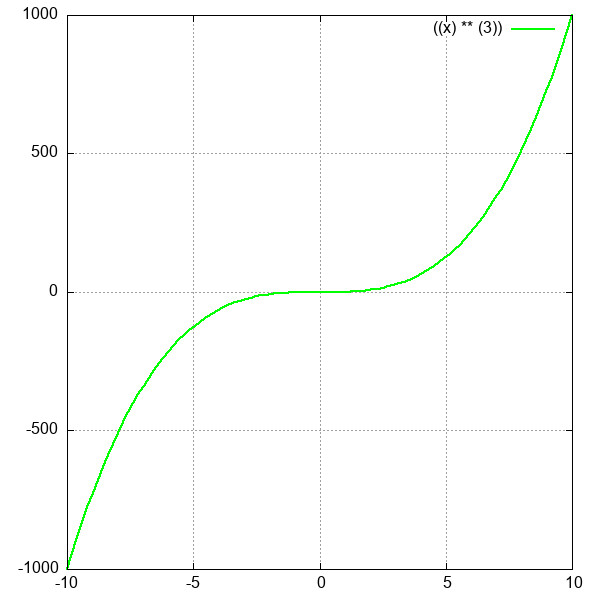
\includegraphics{GraphicDumps/plot.jpg}\newpage \textbf{\LARGE{Глава II. Визуальный анализ функции}}

Ну ты же всё равно не будешь это проверять

\begin{center}
$y = $$(sin(x)+cos(x)) \cdot 2$

\end{center}
\newpage \textbf{\LARGE{Глава III. Дифференцирование}}

Поэтому

\begin{center}
 ($x)'
  = 1$\end{center}
В ближайшее время ожидаются осадки из ваших слёз от попыток понять этот переход

\begin{center}
 ($sin(x))'
  = 1 \cdot cos(x)$\end{center}
Хорошо там, где производной нет\cite{link2}

\begin{center}
 ($x)'
  = 1$\end{center}
Автору приснилось, что следующее преобразование верно

\begin{center}
 ($cos(x))'
  = 1 \cdot (0-sin(x))$\end{center}
Хорошо там, где производной нет\cite{link2}

\begin{center}
 ($sin(x)+cos(x))'
  = 1 \cdot cos(x)+1 \cdot (0-sin(x))$\end{center}
По лемме $\sqrt{-759}$
\begin{center}
 ($2)'
  = 0$\end{center}
Как будет доказано в следующем семестре

\begin{center}
 ($(sin(x)+cos(x)) \cdot 2)'
  = (1 \cdot cos(x)+1 \cdot (0-sin(x))) \cdot 2+(sin(x)+cos(x)) \cdot 0$\end{center}
\newpage \textbf{\LARGE{Глава IV.Упрощение выражения}}

Обоснование этого пререхода предостовляется читателю в качестве несложного упрожнения

\begin{center}
$1 \cdot cos(x) = cos(x)$\end{center}
Хорошо там, где производной нет\cite{link2}

\begin{center}
$1 \cdot (0-sin(x)) = 0-sin(x)$\end{center}
Я придумал поистине удивительное доказательство этого факта, но поля этой книги слишком малы\ldots

\begin{center}
$(sin(x)+cos(x)) \cdot 0 = 0$\end{center}
Очевидно, что

\begin{center}
$(cos(x)+(0-sin(x))) \cdot 2+0 = (cos(x)+(0-sin(x))) \cdot 2$\end{center}
\newpage \textbf{\LARGE{Глава V. Полученая производная}}

$y = $$(sin(x)+cos(x)) \cdot 2$

$y' = $$(cos(x)+(0-sin(x))) \cdot 2$

\includegraphics{GraphicDumps/plot_1.jpg}\newpage \textbf{\LARGE{Глава VI. Разложение функции по формуле Тейлора}}

Функция производной не стоит\cite{link2}

\begin{center}
\end{center}
\begin{center}$sin(1) = 0.841471$\end{center}
Имеем

\begin{center}
\end{center}
\begin{center}$cos(1) = 0.540302$\end{center}
Дифференциал от производной не далеко падает\cite{link2}

\begin{center}
\end{center}
\begin{center}$0.841471+0.540302 = 1.38177$\end{center}
Продвинутый читатель уже заметил, что

\begin{center}
\end{center}
\begin{center}$1.38177 \cdot 2 = 2.76355$\end{center}
По лемме $\sqrt{-759}$
\begin{center}
 ($x)'
  = 1$\end{center}
Спешка нужна только в армии и при ловле блох. Но не как уж ни при вычислении производной\cite{link2}

\begin{center}
 ($sin(x))'
  = 1 \cdot cos(x)$\end{center}
Как было показано ранее

\begin{center}
 ($x)'
  = 1$\end{center}
Говорят

\begin{center}
 ($cos(x))'
  = 1 \cdot (0-sin(x))$\end{center}
Единственное, что я не понимаю, так это то, зачем ты это читаешь

\begin{center}
 ($sin(x)+cos(x))'
  = 1 \cdot cos(x)+1 \cdot (0-sin(x))$\end{center}
Segmentation fault (core dumped)

\begin{center}
 ($2)'
  = 0$\end{center}
Откуда

\begin{center}
 ($(sin(x)+cos(x)) \cdot 2)'
  = (1 \cdot cos(x)+1 \cdot (0-sin(x))) \cdot 2+(sin(x)+cos(x)) \cdot 0$\end{center}
Очевидно, что

\begin{center}
$1 \cdot cos(x) = cos(x)$\end{center}
Ну вот как этот матан тебе в жизни пригодится?

\begin{center}
$1 \cdot (0-sin(x)) = 0-sin(x)$\end{center}
ИИИИЕЕЕЕсли\cite{link3}

\begin{center}
$(sin(x)+cos(x)) \cdot 0 = 0$\end{center}
ИИИИЕЕЕЕсли\cite{link3}

\begin{center}
$(cos(x)+(0-sin(x))) \cdot 2+0 = (cos(x)+(0-sin(x))) \cdot 2$\end{center}
Имеем

\begin{center}
\end{center}
\begin{center}$cos(1) = 0.540302$\end{center}
Отметим, что

\begin{center}
\end{center}
\begin{center}$sin(1) = 0.841471$\end{center}
Первая производная комом\cite{link2}

\begin{center}
\end{center}
\begin{center}$0-0.841471 = -0.841471$\end{center}
//TODO: Лёша, придумай переход. У меня идеи закончились

\begin{center}
\end{center}
\begin{center}$0.540302+-0.841471 = -0.301169$\end{center}
Дифференциал Елена всего в 100 метрах от вас...

\begin{center}
\end{center}
\begin{center}$-0.301169 \cdot 2 = -0.602337$\end{center}
Не трудно заметить

\begin{center}
\end{center}
\begin{center}$\frac{-0.602337}{1} = -0.602337$\end{center}
Поэтому

\begin{center}
$(x-1)^{1} = x-1$\end{center}
От коробки до нк все знают, что

\begin{center}
 ($x)'
  = 1$\end{center}
Если вы понимаете данный переход, то я вам сочувствую

\begin{center}
 ($cos(x))'
  = 1 \cdot (0-sin(x))$\end{center}
Функция производной не стоит\cite{link2}

\begin{center}
 ($0)'
  = 0$\end{center}
Здесь могла быть ваша реклама

\begin{center}
 ($x)'
  = 1$\end{center}
Не трудно заметить

\begin{center}
 ($sin(x))'
  = 1 \cdot cos(x)$\end{center}
Спешка нужна только в армии и при ловле блох. Но не как уж ни при вычислении производной\cite{link2}

\begin{center}
 ($0-sin(x))'
  = 0-1 \cdot cos(x)$\end{center}
Британские учёные доказали, что для поддержания мозга в тонусе необходимо ежедневно дифференцировать. Продолжим наше приобщение к здоровому образу жизниn

\begin{center}
 ($cos(x)+(0-sin(x)))'
  = 1 \cdot (0-sin(x))+(0-1 \cdot cos(x))$\end{center}
Хорошо там, где производной нет\cite{link2}

\begin{center}
 ($2)'
  = 0$\end{center}
Автору приснилось, что следующее преобразование верно

\begin{center}
A = $(1 \cdot (0-sin(x))+(0-1 \cdot cos(x))) \cdot 2$\end{center}
\begin{center}
 ($(cos(x)+(0-sin(x))) \cdot 2)'
  = A+(cos(x)+(0-sin(x))) \cdot 0$\end{center}
Здесь могла быть ваша реклама

\begin{center}
$1 \cdot (0-sin(x)) = 0-sin(x)$\end{center}
Дифференциал Елена всего в 100 метрах от вас...

\begin{center}
$1 \cdot cos(x) = cos(x)$\end{center}
Обоснование этого перехода было забанено редактурой

\begin{center}
$(cos(x)+(0-sin(x))) \cdot 0 = 0$\end{center}
При этом

\begin{center}
$((0-sin(x))+(0-cos(x))) \cdot 2+0 = ((0-sin(x))+(0-cos(x))) \cdot 2$\end{center}
Дифференциал от производной не далеко падает\cite{link2}

\begin{center}
\end{center}
\begin{center}$sin(1) = 0.841471$\end{center}
Обоснование этого пререхода предостовляется читателю в платном DLC

\begin{center}
\end{center}
\begin{center}$0-0.841471 = -0.841471$\end{center}
Обоснование этого пререхода предостовляется читателю в платном DLC

\begin{center}
\end{center}
\begin{center}$cos(1) = 0.540302$\end{center}
Для любого эпсилон больше нулю очевидно, что

\begin{center}
\end{center}
\begin{center}$0-0.540302 = -0.540302$\end{center}
Любовь - это верить в его выводы без доказательств...

\begin{center}
\end{center}
\begin{center}$-0.841471+-0.540302 = -1.38177$\end{center}
Телец в козероге, поэтому

\begin{center}
\end{center}
\begin{center}$-1.38177 \cdot 2 = -2.76355$\end{center}
Дураку понятно, что

\begin{center}
\end{center}
\begin{center}$\frac{-2.76355}{2} = -1.38177$\end{center}
Дифференциал Елена всего в 100 метрах от вас...

\begin{center}
 ($0)'
  = 0$\end{center}
Не трудно заметить

\begin{center}
 ($x)'
  = 1$\end{center}
При этом

\begin{center}
 ($sin(x))'
  = 1 \cdot cos(x)$\end{center}
При этом

\begin{center}
 ($0-sin(x))'
  = 0-1 \cdot cos(x)$\end{center}
Ребята не стоит разбираться в этом переходе. Вы молодые, шутливые, вам все легко. Это не то. Это не Чикатило и даже не архивы спецслужб. Сюда лучше не лезть. Серьезно, любой из вас будет жалеть. Лучше закройте тему и забудьте что тут писалось. Я вполне понимаю что данным сообщением вызову дополнительный интерес, но хочу сразу предостеречь пытливых - стоп. Остальных просто не найдут.

\begin{center}
 ($0)'
  = 0$\end{center}
Доказательство данного факта предоставлено лицом или организацией исполняющей функции иностанного агента

\begin{center}
 ($x)'
  = 1$\end{center}
Руководствуясь сборником <<Задачи для подготовки к поступлению в советские ясли>>\cite{link1}

\begin{center}
 ($cos(x))'
  = 1 \cdot (0-sin(x))$\end{center}
Используя выводы из теоремы 1000-7 получаем

\begin{center}
 ($0-cos(x))'
  = 0-1 \cdot (0-sin(x))$\end{center}
Если посмотреть на выражение под другим углом, можно получить

\begin{center}
 ($(0-sin(x))+(0-cos(x)))'
  = (0-1 \cdot cos(x))+(0-1 \cdot (0-sin(x)))$\end{center}
Дураку понятно, что

\begin{center}
 ($2)'
  = 0$\end{center}
Дураку понятно, что

\begin{center}
A = $(0-1 \cdot cos(x))+(0-1 \cdot (0-sin(x)))$\end{center}
\begin{center}
 ($((0-sin(x))+(0-cos(x))) \cdot 2)'
  = (A) \cdot 2+((0-sin(x))+(0-cos(x))) \cdot 0$\end{center}
Руководствуясь базовой логикой, получаем

\begin{center}
$1 \cdot cos(x) = cos(x)$\end{center}
По лемме $\sqrt{-759}$
\begin{center}
$1 \cdot (0-sin(x)) = 0-sin(x)$\end{center}
Без комментариев\cite{link4}

\begin{center}
$((0-sin(x))+(0-cos(x))) \cdot 0 = 0$\end{center}
Функция производной не стоит\cite{link2}

\begin{center}
$((0-cos(x))+(0-(0-sin(x)))) \cdot 2+0 = ((0-cos(x))+(0-(0-sin(x)))) \cdot 2$\end{center}
Дифференциал Елена всего в 100 метрах от вас...

\begin{center}
\end{center}
\begin{center}$cos(1) = 0.540302$\end{center}
Доказательство данного факта предоставлено лицом или организацией исполняющей функции иностанного агента

\begin{center}
\end{center}
\begin{center}$0-0.540302 = -0.540302$\end{center}
От коробки до нк все знают, что

\begin{center}
\end{center}
\begin{center}$sin(1) = 0.841471$\end{center}
Имеем

\begin{center}
\end{center}
\begin{center}$0-0.841471 = -0.841471$\end{center}
Здесь могла быть ваша реклама

\begin{center}
\end{center}
\begin{center}$0--0.841471 = 0.841471$\end{center}
Ты же продолжаешь читать, да?

\begin{center}
\end{center}
\begin{center}$-0.540302+0.841471 = 0.301169$\end{center}
Ребята не стоит разбираться в этом переходе. Вы молодые, шутливые, вам все легко. Это не то. Это не Чикатило и даже не архивы спецслужб. Сюда лучше не лезть. Серьезно, любой из вас будет жалеть. Лучше закройте тему и забудьте что тут писалось. Я вполне понимаю что данным сообщением вызову дополнительный интерес, но хочу сразу предостеречь пытливых - стоп. Остальных просто не найдут.

\begin{center}
\end{center}
\begin{center}$0.301169 \cdot 2 = 0.602337$\end{center}
Дураку понятно, что

\begin{center}
\end{center}
\begin{center}$\frac{0.602337}{6} = 0.10039$\end{center}
\textbf{\LARGE{Получим разложение по формуле Тейлора:}}
\begin{center}
$y = $$2.76355+(-0.602337 \cdot (x-1)+(-1.38177 \cdot (x-1)^{2}+0.10039 \cdot (x-1)^{3}))$$ + o(x^{3})$
\end{center}
\newpage\begin{thebibliography}{}
\bibitem{link1}  "A Synopsis of Elementary Results in Pure and Applied Mathematics"
\bibitem{link2}  "Сборник пословиц и поговорок кафедры высшей математики"
\bibitem{link3}  "Полное собрание лучших высказываний преподавателей МФТИ"
\bibitem{link4}  "Словарь фраз не несущих смысловой нагрузки кафедры философии. 17 издание"
\end{thebibliography}\end{document}